%%%%%%%%%%%%%%%%%%%%%%%%%%%%%%%%%%%%%%%%%%
\section{Part 2 - Exercise 1 - slide 41}
%%%%%%%%%%%%%%%%%%%%%%%%%%%%%%%%%%%%%%%%%%
%
\begin{equation*}
    \min_{\bs x \in \Rbb^{30}} \sqrt{\bs x^\top \bs{Qx} + 
    2 \bs b^\top \bs x + c} + 0.2 \norm{\bs{Dx+\bs 1}}{1},
\end{equation*}
%
where $\bs Q \in \Rbb^{30\times 30}$, $\bs b\in \Rbb^{30}$, $c\in \Rbb$, $\bs D
\in \Rbb^{30\times 30}$. The matrix $\bs Q$ is positive definite. \\

\indent (a) The first step of the problem is to show it is well-defined (i.e. $\bs x^\top \bs{Qx} + 
2 \bs b^\top \bs x + c\geq 0$ if $c> \bs b^\top\bs Q^{-1} \bs b$.). To that aim, letting the Cholesky factorisation of $\bs Q$ being denoted as $\bs Q = \bs L^\top \bs L$, 
\begin{align*}
	\bs x^\top \bs{Qx} + 
2 \bs b^\top \bs x + c &= \bs x^\top \bs{Qx} + \bs b^\top \bs L^{-1} \bs{Lx} + \bs x^\top \bs L^\top \bs L^{-\top} \bs b + \bs b^{\top} \bs L^{-1} \bs L^{-\top} \bs b - \bs b^\top \bs L^\top \bs L^{-\top} \bs b + c,\\
&= \left \| \bs{Lx} + \bs L^{-\top} \bs b \right \|_2^2 + c -\bs b^\top\bs Q^{-1} \bs b. 
\end{align*}  
From the above, as a norm is always nonnegative, one can conclude the problem is well-defined if $c> \bs b^\top\bs Q^{-1} \bs b$.   \\
%
\indent (b) Starting from the norm expression, one can obtain 
\begin{align*}
	\sqrt{\bs x^\top \bs{Qx} + 
    2 \bs b^\top \bs x + c} + 0.2 \norm{\bs{Dx+\bs 1}}{1} &= \left \| \begin{matrix}
    \bs{Lx} + \bs L^{-\top} \bs b \\
    \\
    \sqrt{c -\bs b^\top\bs Q^{-1} \bs b}
    \end{matrix} \right \|_2 + 0.2 \norm{\bs{Dx+\bs 1}}{1}. 
\end{align*}
As a norm is convex, as a composition with a  linear mapping preserves convexity and since a sum of convex functions is convex, the problem is convex. \\
\indent (c) To fit the framework of FISTA,  we denote by $f(\bs x) = \sqrt{\bs x^\top \bs{Qx} + 
2 \bs b^\top \bs x + c}$ and $g(\bs x) =  0.2 \norm{\bs{Dx+\bs 1}}{1}$ where $g$ is 
proper, closed and convex, and $f$ is $L_f$-smooth and convex. 
More precisely, the Lipschitz constant of $f$ can be identified by computing its 
Hessian: 
\begin{align*}
\bs \nabla f(\bs x) & = \frac{\bs{Qx}+\bs b}{\sqrt{\bs x^\top \bs{Qx} + 
2 \bs b^\top \bs x + c}}, \\
\bs \nabla^2 f(\bs x) & = \frac{\bs Q}{\sqrt{\bs x^\top \bs{Qx} + 
2 \bs b^\top \bs x + c}} - \frac{(\bs{Qx}+\bs b)(\bs{Qx}+\bs b)^\top}{\left(\bs x^\top \bs{Qx} + 
2 \bs b^\top \bs x + c\right)^{\frac{3}{2}}}. 
\end{align*}
The latter can be bounded as 
\begin{align*}
	\bs \nabla^2 f(\bs x) \preceq  \frac{\bs Q }{\sqrt{\bs x^\top \bs{Qx} + 
2 \bs b^\top \bs x + c}} = \frac{\bs Q }{ \sqrt{c -\bs b^\top\bs Q^{-1} \bs b} \sqrt{1+\frac{\left \| \bs{Lx} + \bs L^{-\top} \bs b \right \|_2^2}{ c -\bs b^\top\bs Q^{-1} \bs b}}} \preceq \frac{\bs Q }{ \sqrt{c -\bs b^\top\bs Q^{-1} \bs b}},
\end{align*}
leading to $L_f = \frac{\lambda_{\text{max}}\left(\bs Q\right)}{\sqrt{c -\bs b^\top\bs Q^{-1} \bs b}}$. In the case of the exercise, we obtain $L_f = 53.54$ and thus a step size of  $0.019$. \\
As $\bs D \bs D^\top = \bs I$, one can compute the proximal operator of $\alpha g$ as 
\begin{align*}
	\prox_{\alpha g}(\bs x) & = \bs x + \bs D^\top \left( 
\soft{0.2\alpha} (\bs{Dx}+\bs 1) - \bs{Dx} - \bs 1 \right),\\
 & =  \bs D^\top 
\soft{0.2\alpha} (\bs{Dx}+\bs 1) -\bs D^\top \bs 1 .
\end{align*}
This leads to 
\begin{itemize}
    \item (\emph{Proximal gradient}):
    \begin{align*}
    \begin{split}
        \bs x^{k+1} &= \prox_{\tinv{L_f}g} (\bs x^k - \tinv{L_f} \nabla f(\bs x^k)) \\ 
        &=  \bs D^\top 
       \soft{\frac{0.2}{L_f}} \left[ \bs D(\bs x^k - \tinv{L_f} \nabla 
        f(\bs x^k) ) + \bs 1 \right]  - \bs D^\top  \bs 1    \\
        &= \bs D^\top  \soft{\frac{0.2}{L_f}} \left[ 
        \bs D(\bs x^k - \tinv{L_f} \frac{\bs{Qx}^k+\bs b}{\sqrt{(\bs x^k)^\top 
        \bs{Qx}^k + 2 \bs b^\top \bs x^k + c}} ) + \bs 1 \right] - \bs D^\top \bs 1 .
    \end{split}
    \end{align*}
    
    \item (\emph{FISTA}):
      \begin{align*}
    \begin{split}
    \left\{
    \begin{array}{lll}
        \bs x^{k+1} &= \bs D^\top  \soft{\frac{0.2}{L_f}} \left[ 
        \bs D(\bs y^k - \tinv{L_f} \frac{\bs{Qy}^k+\bs b}{\sqrt{(\bs y^k)^\top 
        \bs{Qy}^k + 2 \bs b^\top \bs y^k + c}} ) + \bs 1 \right] - \bs D^\top \bs 1 \\
        t_{k+1} &= \frac{1+\sqrt{1+4t_k^2}}{2} \\
        \bs y^{k+1} &= \bs x^{k+1} + \left( 
        \frac{t_k-1}{t_{k+1}} \right) (\bs x^{k+1}- \bs x^k)
    \end{array}
    \right.
    \end{split}
    \end{align*}
\end{itemize}
Implementing both methods, their objective values along the iterations are displayed in \Cref{fig:ex1}. To get a more precise view, their objective values at iterations $1$, $101$, ..., $1001$ are the following:
\begin{align*}
	F\left(\bs x^{k,\text{PG}}\right)&= [55.543, 46.768, 45.150 , 44.398, 44.116, 44.007, 43.940 , 43.894,
       43.862, 43.840 , 43.826],\\
       F\left(\bs x^{k,\text{FISTA}}\right)&= [55.543, 43.811, 43.772, 43.771, 43.770 , 43.770 , 43.770 , 43.770 ,
       43.770 , 43.770 , 43.770 ]  .     
\end{align*}
\begin{figure}[H]
    \centering
    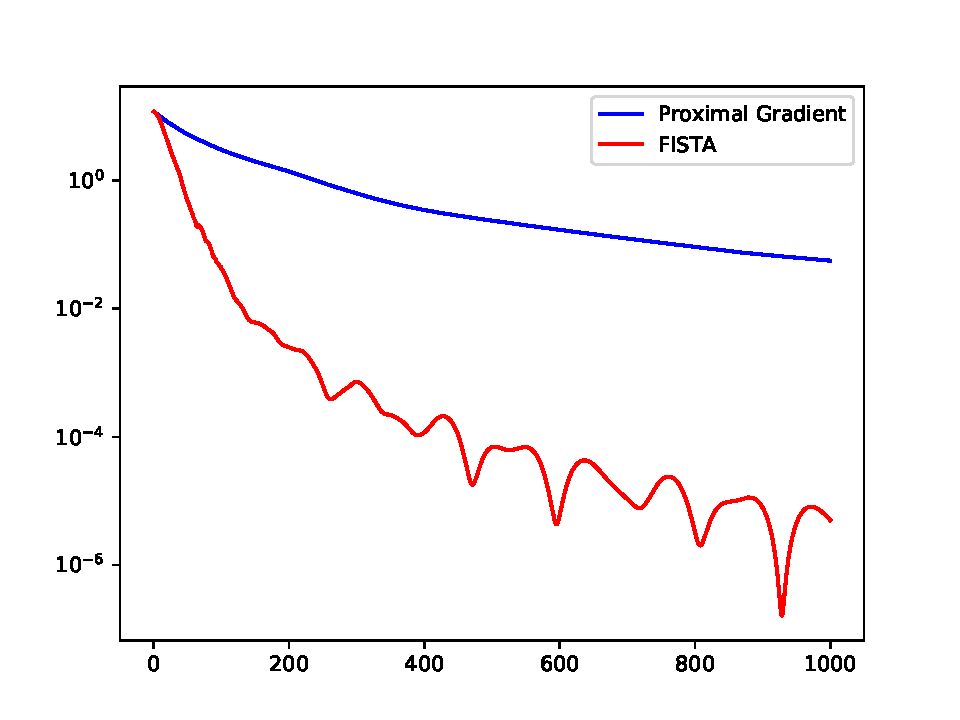
\includegraphics[width=14cm]{images/part2_ex1.pdf}
    \caption{$F(\bs x^k)-F_{\text{opt}}$ in log-scale along the 
  y-axis for the first 1001 iterations of each of the methods 
  with all-zeros vectors and a constant stepsize. The optimal solution has been computed as the best one across 10000 iterations.  }
  \label{fig:ex1}
\end{figure}
Finally, the vectors found by both methods after $1001$ iterations are the following:
       \begin{align*}
       \bs x^{*,\text{PG}} &= [0.406, -0.093, -0.093, -0.874, -1.025, -0.044,  0.521, -1.16 ,
        0.877,  0.129, -0.242,  1.664,  1.32 , -0.561, -0.079, -1.764,\\& \qquad 
       -1.351, -0.387, -1.158,  0.844,  0.43 , -0.715, -0.349, -0.037,
        1.408, -0.971,  1.206,  0.795,  0.568,  1.284],\\
        \bs x^{*,\text{FISTA}} &= [-0.455, -0.389,  0.291, -1.149, -1.309, -0.43 ,  0.667, -1.434,
        1.082, -0.019, -0.416,  1.732,  1.293, -0.541, -0.143,\\& \qquad  -1.704,
       -1.396, -0.742, -1.539,  0.335, -0.218, -0.662, -0.151, -0.085,
        1.801, -0.566,  1.321,  0.849,  0.701,  1.091].
       \end{align*}
        


%
%%%%%%%%%%%%%%%%%%%%%%%%%%%%%%%%%%%%%%%%%%
\section{Part 2 - Exercise 3 - slides 71-72}
%%%%%%%%%%%%%%%%%%%%%%%%%%%%%%%%%%%%%%%%%%
%
Given a set of data points $\bs x_1, \bs x_2,\cdots,\bs x_n \in \Rbb^d$ and 
corresponding labels $y_1,y_2,\cdots,y_n$. The soft margin SVM problem is given 
by 
\begin{equation*}
    \min \left\{\tinv 2\norm{\bs w}{2}^2+C \sum_{i=1}^{n} \max 
    \left\{0,1-y_i \bs w^\top \bs x_i\right\}\right\}
\end{equation*}

\indent (a) Letting $f(\bs w) = \tinv 2\norm{\bs w}{2}^2$, $g(\bs z) = C\sum_{i=1}^n\max\left(0,1-z_i\right)$, and $\bs A = \begin{bmatrix}
	\bs x_1y_1\\ \vdots \\ \bs x_ny_n
\end{bmatrix}$, the problem matches the canonical form 
\begin{align*}
	\min f(\bs w) + g(\bs{Aw}),
\end{align*}
with $f$ proper closed and $\sigma$-strongly convex (here $\sigma=1$), $g$ proper closed and convex. Hence, the Dual Proximal Gradient (DPG) or the Fast DPG (FDPG) methods can be applied. To that aim,
the following optimisation problem must be solved. 
\begin{align*}
	\underset{\bs w}{\text{argmax}} \left\{\left \langle \bs w, \bs A^\top \bs y \right \rangle - f(\bs w)\right\} &= \underset{\bs w}{\text{argmax}} \left\{\left \langle \bs w, \bs A^\top \bs y \right \rangle - \tinv 2\norm{\bs w}{2}^2 \right\} = \bs A^\top \bs y. 
\end{align*}
Also, we compute the proximal operator of $\eta g$ as 
\begin{align*}
	\text{prox}_{\kappa \max(0,1-x)}(x) &= 1-\text{prox}_{\kappa \max(0,x)}(1-x),\\
	&= 1-\text{prox}_{\kappa \sigma_{[0;1]}}(1-x),\\
	&= x+\min\left\{\max\left\{1-x,0\right\},\kappa\right\}.
\end{align*}
This leads to the compact formulation 
\begin{align*}
	\text{prox}_{\eta g}(\bs w)= \bs w+\min\left\{\max\left\{1-\bs w,0\right\},\eta C\right\}.
\end{align*}
Plugging these expressions into the DPG and FDPG  iterations, one obtains 
\begin{itemize}
    \item (\emph{DPG}):
    \begin{align*}
    \begin{split}
    \left\{
    \begin{array}{ll}
   & \bs x^{k} = \bs A^\top \bs y^k\\
        &\bs y^{k+1} = \min\left\{\max\left\{\bs y^k-\tinv L\bs A \bs x^k + \tinv L,0\right\}, C\right\}. \end{array}
   \right. \end{split}
    \end{align*}
    
    \item (\emph{FDPG}):
      \begin{align*}
    \begin{split}
    \left\{
    \begin{array}{ll}
         \bs u^{k} &= \bs A^\top \bs w^k\\
        \bs y^{k+1} &= \min\left\{\max\left\{\bs w^k-\tinv L\bs A \bs u^k + \tinv L,0\right\}, C\right\}\\
        t_{k+1} &= \frac{1+\sqrt{1+4t_k^2}}{2} \\
        \bs w^{k+1} &= \bs y^{k+1} + \left( 
        \frac{t_k-1}{t_{k+1}} \right) (\bs y^{k+1}- \bs y^k)
    \end{array}
    \right.
    \end{split}
    \end{align*}
    and with  $\bs x^k = \bs A^\top \bs y^k$.
\end{itemize}
%

\indent (b) Both methods have been implemented. As it was not given in the exercise, we have assumed $C=1$. Also, the class information (originally equal to $1$ or $2$) has been transformed in to $-1$ and $1$ as this is the setup of usual SVM. Finally, comparing the problem formulation with SVM, we have concluded the obtained hyperplane was assumed to go through the origin. This leads to the results displayed in \Cref{fig:ex3}, were one can observe two points are actually classified incorrectly. 
\begin{figure}[H]
    \centering
    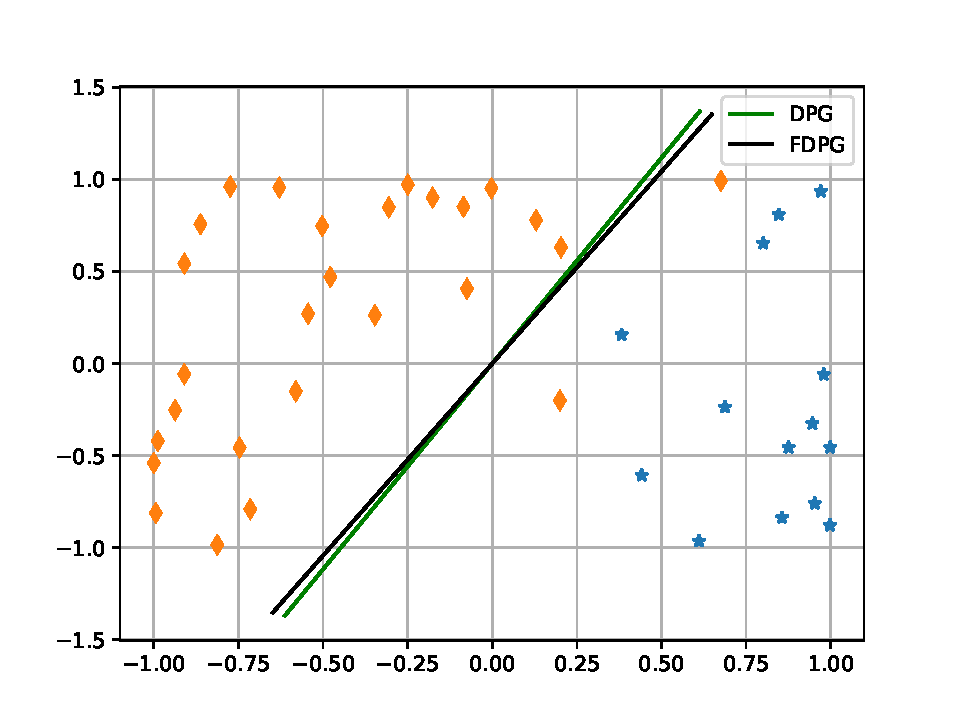
\includegraphics[width=14cm]{images/part2_ex3.pdf}
    \caption{Separating hyperplanes obtained by both methods.   }
  \label{fig:ex3}
\end{figure}
More precisely, the vectors obtained by both methods after $40$ iterations are the following. 
       \begin{align*}
       \bs x^{*,\text{DPG}} &= [-2.040, 0.913],\\
        \bs x^{*,\text{FDPG}} &= [-2.124,1.012].
       \end{align*}


